\documentclass[12pt]{report}

\usepackage[italian]{babel}
\usepackage[latin1]{inputenc}
\usepackage{url}
\usepackage{biblatex}
\usepackage{amsmath}
\usepackage{graphicx}
\usepackage{caption}

\bibliography{bib}

\title {IaasFog}
\author{Stefano Cadario, Luca Cavazzana}
\data{\date}

\begin{document}
\maketitle

\tableofcontents

\chapter{Introduzione}

\noindent L'obbiettivo del progetto \`e estrarre un parametro numerico indicante la visibilit\`a in caso di nebbia utilizzando esclusivamente delle immagini riprese da una telecamera montata su una automobile.\\
La tecnica utilizzata si basa sull'analisi della variazione del contrasto delle features individuate in ogni frame dell'immagine con il fine di trovare il parametro $\lambda$ della funzione $$ke^{-t/\lambda}$$ Tale funzione deriva da una prima analisi teorica del problema in questione: il parametro $\lambda$ infatti rappresenta il tempo medio d'impatto di una feature che sta emergendo dalla nebbia, per cui il valore di contrasto viene considerato come pari a $k/e$.\\
I problemi affrontati nel corso di questo progetto consistono nello sviluppo di una tecnica performante per l'individuazione e il tracking di features il cui movimento relativo sia consistente con quello del veicolo, e trovare un metodo per il calcolo del contrasto e la stima del parametro in questione sufficientemente robusto al livello di rumore sui dati.\\
	 	
\noindent Un simile sistema potrebbe essere integrato fra i sensori di un veicolo, monitorando l'idoneit\`a della velocit\`a di crociera rispetto alle condizioni di visibilit\`a e ai tempi di reazione del conducente. Nel campo emergente dei veicoli autonomi similmente potrebbe vincolare il valore massimo di velocit\`a in base ai tempi di risposta, oppure potenziare la consapevolezza del sistema di analisi fornendo un parametro per la stima della rumorosit\`a/bont\`a dei dati a seconda della distanza dell'elemento da cui sono state ricavati.

\chapter{Qualche titolo}

\section{Tracking delle features}

\noindent Il tracking delle features deve contemporaneamente individuare il maggior numero di features in ogni immagine ma nel contempo escludere gli outliers che influirebbero nei passaggi successivi dell'elaborazione.\\
L'elaborazione dei frame avviene in modo inverso rispetto al tempo perch\'e in questo modo si \`e in grado di individuare le features quando sono ben visibili per poi inseguirle nei frame temporalmente precedenti, dove il riconoscimento \`e pi\`u difficoltoso a causa della nebbia.\\

\noindent Ad ogni frame viene eseguita la funzione \verb|cvGoodFeaturesToTrack| che individua la posizione di features con autovalori pi\`u alti e quindi con maggior probabilit\`a di essere individuati nei frame successivi. Nel frame successivo vengono quindi cercate le stesse features individuate fin'ora utilizzando la funzione \verb|cvCalcOpticalFlowPyrLK|, che utilizzando l'algoritmo iterativo di \emph{Lucas-Kanade}~\cite{lucaskanade81} ricalcola la nuova posizione di ogni feature.\\

\noindent Prima di aggiungere alla sequenza il nuovo punto individuato vengono effettuati dei controlli di coerenza: la nuova posizione deve avere direzione concorde con i punti antecedenti ed il nuovo passo deve essere maggiore dei precedenti. Una sequenza di features \`e considerata valida se \`e inseguita per almeno cinque frame (essendo quattro il numero minimo necessario per il calcolo del birapporto), in caso contrario viene eliminata. Se la feature \`e valida viene eseguito un controllo sulla cross-ratio dei punti che deve essere prossima a 4/3. I punti trovati saranno comunque soggetti ad errori di posizione dovuti a diversi fattori e quindi non collineari: per rimediare viene quindi calcolata la retta di regressione, su cui verranno proiettati i punti per l'analisi del birapporto.\\

\noindent Il tracking di feature diventa sempre pi\`u difficoltoso all'avvicinarsi al vanishing point a causa del calo dei livelli di contrasto causati dalla nebbia che riduce la possibilit\`a di individuazione; per ovviare a questo problema vengono calcolate le posizioni teoriche delle features utilizzando i punti nei frame precedenti e la cross-ratio nota. Il tracking di una feature ha termine quando non si hanno pi\`u frame disponibili oppure quando lo step del nuovo punto \`e inferiore ai $0.5$ pixel.

\section{Calcolo vanishing point}
\noindent La posizione del vanishing point riveste un ruolo fondamentale nella risoluzione del problema poich\'e viene coinvolto sia nel filtro di outliers, sia nel calcolo del tempo d'impatto di ogni feature.\\

\noindent Inizialmente \`e stato implementato un algoritmo che prevedeva l'individuazione di tutti i punti di intersezione tra rette e da questi ricavare il punto che minimizza la distanza con tutti gli altri. Questo approccio, sebbene abbia dato buoni risultati, si \`e rivelato troppo lento a causa della complessit\`a eccessiva del problema che richiedeva fino a $15$ secondi di elaborazione per $200$ features.\\

\noindent Dopo un primo tentativo di ottimizzare l'algoritmo esistente si \`e deciso di riscriverlo sfruttando RANSAC:
\begin{itemize}
	\item	Ad ogni iterazione viene eletto casualmente un possibile candidato vanishing point calcolando l'intersezione delle rette rappresentanti due features, con il solo vincolo di essere all'interno del field of view dell'immagine.
	\item	Per ogni retta viene calcolata la distanza dal vanishing point candidato. A tale distanza viene assegnato un punteggio (da 0 a 1) che sommato a quelli di ogni retta determina il rank del candidato vanishing point.
	\item	Se il nuovo vanishing point ha un rank migliore dei precedenti viene eletto come nuovo best vanishing point.
	\item	Il ciclo termina quando vengono analizzati un numero di intersezioni ritenuto sufficiente (circa il $5\%$ di tutte le possibili intersezioni tra rette).
\end{itemize}

\noindent L'algoritmo applicato a diversi set di dati ha restituito buoni risultati con tempi notevolmente ridotti (circa 1 secondo di elaborazione per 200 features) rispetto alla prima implementazione meno efficiente.\\

\noindent La posizione del vanishing point reale viene poi affinata utilizzando SVD con il $50\%$ delle rette pi\`u vicine al vanishing point trovato in precedenza. 

\section{Calcolo del tempo all'impatto}

\noindent Dato un set di punti di coordinate $A$ e $B$, rappresentante una stessa feature in differenti immagini e conoscendo il framerate $f$ delle telecamera \`e possibile calcolare il tempo d'impatto, ossia l'istante in cui la feature attraverser\`a il piano immagine mediante il birapporto

$$ cross(i,a,b,v) = \frac{\overline{ia}}{\overline{ab}}\frac{\overline{av}}{\overline{iv}} = \frac{\overline{i'a'}}{\overline{a'b'}}\frac{\overline{a'v'}}{\overline{i'v'}} $$

\noindent Essendo nel mondo reale le distanze rispetto al vanishing point infinite, come quelle rispetto al piano della telecamera nelle immagini, la formula si semplifica

$$ \frac{\overline{ia}}{\overline{ab}} = \frac{\overline{a'v'}}{\overline{a'b'}} $$

\noindent Dal momento che $\overline{a'v'}$ e $\overline{a'b'}$ sono noti, ed essendo $ab$ la distanza percorsa dal veicolo fra le due immagini ($velocit\`a/framerate$), il tempo d'impatto pu\`o essere ottenuto come

$$ t_{i,b} = \frac{\overline{a'v'}}{\overline{a'b'}}\frac{\overline{ab}}{v} = \frac{\overline{a'v'}}{\overline{a'b'}}*f^{-1} $$

\section{Calcolo del contrasto}
\noindent Per il calcolo delle features sono stati presi in considerazione diversi approcci per il calcolo del contrasto nell'intorno di una feature: oltre alla formule di Michelson e Weber, gi\`a sfruttate nelle precedenti fasi del progetto, \`e stato deciso di introdurre anche Root Mean Square, che calcola il livello di contrasto secondo la formula

$$ c\left(I_{M\times N}\right) = \sqrt{\frac{1}{MN}\sum_{i=1}^N\sum_{j=1}^M(i_{ij}-\bar{I})^2} $$

\noindent Dal momento che nel calcolo del valore contribuiscono tutti i pixel all'interno della finestra tale formula risulta essere molto pi\`u resistente al rumore rispetto alle precendenti, il cui risultato risulta essere dipendente dall'errore sul singolo pixel centrale per Weber, e dall'errore sui valori di min e max per Michelson.\\
Confrontanto i valori ottenti calcolando i livelli di contrasto utilizzando i diversi metodi mostrano come RMS tenda a generare curve pi\`u smooth.

\begin{center}
	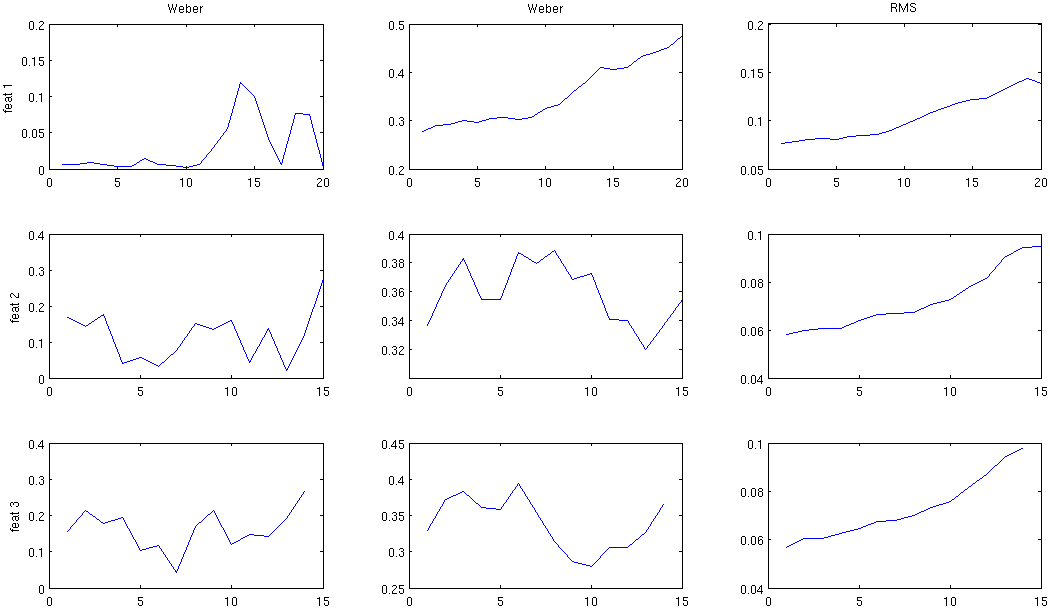
\includegraphics[scale=0.60, angle=90.0]{images/compContr1.png}
	\captionof{figure}{confronto fra i valori di contrasto ottenuti mediante i differenti approcci}
	\label{fig:contr01}
\end{center}
\begin{center}
	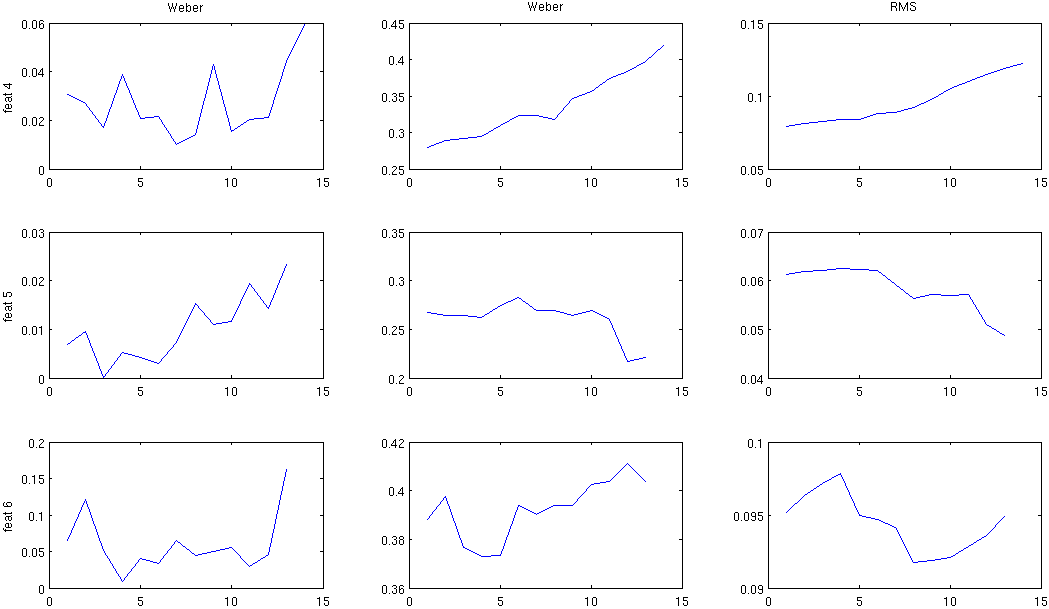
\includegraphics[scale=0.60, angle=90.0]{images/compContr2.png}
	\captionof{figure}{confronto su nuovi set}
	\label{fig:contr02}
\end{center}
\begin{center}
	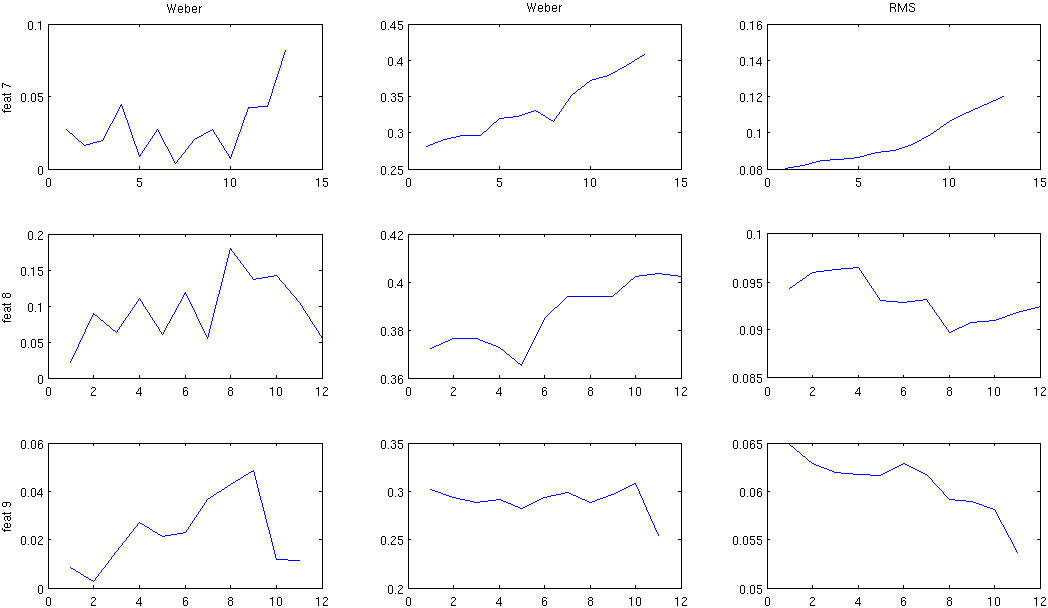
\includegraphics[scale=0.60, angle=90.0]{images/compContr3.png}
	\captionof{figure}{confronto su nuovi set}
	\label{fig:contr03}
\end{center}

\noindent Una particolarit\`a di RMS \`e che, al contrario delle altre tecniche, il risultato dipende dallo spazio di colori utilizzato per rappresentare l'immagine (facilmente aggirabile riscalando rispetto alla profondit\`a del colore).

\section{Stima dei parametri}

\subsection{Stima di $\lambda$ mediante minMax}

\noindent Definiamo la formula del contrasto per ogni feature come

$$ c_{i,s} = k_se^{-t_{i,s}/\lambda} $$

\noindent dove $c_{i,s}$ \`e il livello di contrasto all'istante $t_{i,s}$. Il parametro $k_s$ risulta essere costante all'interno di ogni singola sequenza di feature, mentre $\lambda$ \`e globale.
Sfruttando $k_s$ \`e possibile imporre la seguente uguaglianza fra due campioni nello stesso set

$$ c_1e^{t_1/\lambda} = c_2e^{t_2/\lambda} $$
$$ \lambda = \frac{t_2-t_1}{\log\frac{c_1}{c_2}} $$

\noindent in modo da stimare il parametro $\lambda$ sul singolo set utilizzando i livelli di contrasto massimi e minimi (ed i relativi tempi all'impatto).\\
A questo punto viene introdotto un primo semplice criterio atto ad eliminare set eccessivamente rumorosi: ricordando che i dati sono ordinati sul tempo d'impatto (e quindi il contrasto risulter\`a essere una funzione decrescente), vengono ignorati set in cui la differenza fra gli indici dei valori di contrasto minimo e massimo non \`e sufficientemente grande (nel nostro caso deve essere superiore alla met\`a del numero di feature all'interno del set).\\
Successivamente si pu\`o procedere con il calcolo di un $\lambda$ globale in base a quelli stimati calcolandone la media, mediana o applicando altre tecniche pi\`u complesse.

\subsection{Fitting di $\lambda$}
\noindent Una tecnica adottata \`e stata quella di sfruttare la funzione \verb|fit| di Matlab per estrarre il parametri $k$ e $\lambda_s$ che meglio descrivono ogni singolo inseguimento. Per ogni dato viene cos\`i calcolato l'errore rispetto alla relativa curva generata, valore in base al quale verr\'a eliminata la met\'a dei dati peggiori, mentre l'altra met\'a verr\'a utilizzata per calcolare un refit.\\
Fra i nuovi $\lambda_s$ calcolati viene selezionato il $20\%$ migliore in base ad un valore, calcolato mediante diversi approcci:

\begin{itemize}
	\item	\emph{errore primo/secondo fitting}: c'\`e poco da spiegare. L'errore viene calcolato come media dei rapporti fra l'errore e la proiezione del dato sulla curva.
	\item	\emph{variazione dell'errore}: nell'ipotesi di un buon set di dati la variazione dell'errore medio non dovrebbe essere molto grande. Viene quindi tenuta in considerazione la differenza fra gli errori calcolati (prossima a $0$ per buone features) o il rapporto (prossimo a $1$).
	\item	\emph{differenza curva}: viene calcolata la variazione fra i parametri. Per aggregare i due parametri viene considerata la differenza fra l'area delle due curve, calcolata come $$\left|\int^{\infty}_0\left(k_1e^{-t/\lambda_1} - k_2e^{-t/\lambda_2}\right)dt\right|$$ $$= \left|\left[ k_2\lambda_2e^{-t/\lambda_2} - k_1\lambda_1e^{-t/\lambda_1} \right]^\infty_0\right|$$ $$ = \left|k_2\lambda_2 - k_1\lambda_1\right|$$
\end{itemize}

\noindent L'ultima soluzione appare essere quella pi\`u robusta, e viene quindi utilizzata. Il $\lambda$ globale viene cos\`i calcolato come la mediana di quelli selezionati.

\subsection{Normalizzazione mediante fitting di $k$ e RANSAC}
\noindent Un'altra tecnica sperimentata consiste nello sfruttare tutte le informazioni disponibili  per stimare (mediante la funzione \verb|fit| di Matlab) i parametri $k_s$ e $\lambda_s$ che minimizzano l'errore su ogni singolo set di features.\\
$\lambda_s$, analogamente al metodo precedente, viene sfruttato per eliminare set eccessivamente rumorosi mantenendo solo quelli al di sotto del quantile $0.8$.\\
Il parametro $k_s$ viene invece utilizzato per normalizzare features con un valore di contrasto ``intrinseco'' (ovvero il massimo livello che otterremmo in condizioni idealei, senza nebbia): considerando $c_{i,s}/k_s$ possiamo cos\`i considerare sulla funzione discreta solo il contributo della nebbia, permettondoci di aggregare i dati di diversi set e stimare il parametro $\lambda$ globale sulla formula $$ c(t) = e^{-t/\lambda} $$ mediante RANSAC.\\
Questa implementazione di RANSAC seleziona a caso il $25\%$ dei set disponibili, i cui valori di contrasto vengono aggregati, ordinati in base al tempo d'impatto ed infine usati per stimare il $\lambda$ globale. Per tale parametro verr\'a poi calcolato il set di consenso ed il relativo errore, iterando il processo come da manuale.



\chapter{Conclusione e sviluppi futuri}
\noindent I risultati dei test hanno evidenziato come il problema sia fortemente influenzato dal numero di outliers derivati sia un errato tracking delle features, sia da una non perfetta variazione del contrasto sulle features stesse. Il maggior sforzo computazionale \`e infatti da attribuire alla complessit\`a degli algoritmi utilizzati per escludere gli outliers in tutte le fasi dell'elaborazione in modo da avere dei valori attendibili in ogni condizione.\\

\noindent Sono stati analizzati diversi approcci ed algoritmi per la risoluzione del problema, si \`e preferito in ultimo di sacrificare il tempo di elaborazione in cambio di una migliore affidabilit\`a dei risultati: gli algoritmi utilizzati sono in grado di individuare autonomamente le buone features e scartare quelle meno buone, ottenendo degli ottimi risultati esposti nei capitoli precedenti.\\

\noindent Possibili sviluppi futuri possono riguardare la reimplementazione in C\verb|++| del codice Matlab ed un'ottimizzazione degli algoritmi mirata a migliorarne le performance, eventualmente fino al punto di rendere possibile l'analisi direttamente su di uno streaming video in realtime, senza le rielaborazioni successive del codice attualmente in uso.\\





\chapter{Funzioni}

Viene qui presentata una panoramica delle funzioni realizzate. Per informazioni pi\`u dettagliate circa il loro utilizzo consultare l'\verb|help| delle funzioni~\cite{lucaskanade81}.

\section[C++]{C\verb_++_}

\paragraph*{\verb_FindFeatures:_} main, parsa input e lancia nuFindFeatures

\paragraph*{\verb_nuFindFeatures:_} bla bla bla

\paragraph*{\verb_iaasFindCorners:_} estrae i corner dall'immagine

\paragraph*{\verb_iaasTrackCorners:_} cerca di rintracciare i corner della prima immagine (gi\`a calcolati) nella seconda

\paragraph*{\verb_verifyNewFeatureIsOk:_} verifica che una sequenza di corner sia coerente in base a \dots

\paragraph*{\verb_getAroundContrast:_} calcola il contrasto nell'intorno di una features usando RMS: $$ c\left(I_{M\times N}\right) = \sqrt{\frac{1}{MN}\sum_{i=1}^N\sum_{j=1}^M(i_{ij}-\bar{I})^2} $$

\paragraph*{\verb_verifyValidFeature:_} \dots


\paragraph*{\verb_printFeatures:_} scrive sul file la lista di feature valide come:
\begin{verbatim}
	     primoFrame numeroFrame [xCoord yCoord contrasto]+
\end{verbatim}

\section{Matlab}

\paragraph*{\verb_iaas:_}

\paragraph*{\verb_inspectContrast:_} stampa a video le sequenze di features per un'ispezione visiva.

\paragraph*{\verb_inspectFeatures:_}

\paragraph*{\verb_estimateLamFit:_}

\paragraph*{\verb_fitLamContr:_}

\paragraph*{\verb_fitNormContr:_}

\paragraph*{\verb_myRansac:_} implementazione di RANSAC per calcolare il parametro lambda della funzione del contrasto dati in ingresso dei set di features normalizzati.

\paragraph*{\verb_compareContrast:_}

\paragraph*{\verb_MichelsonContrast:_} date le coordinate di una feature e la relative immagine restituisce il livello di contrasto nell'intorno come $$c\left(I\right) = \frac{\max(I)-\min(I)}{\max(I)+\min(I)}$$

\paragraph*{\verb_rsmContrast:_} date le coordinate di una feature e la relativa immagine calcola il livello di contrasto nell'intorno come $$ c\left(I_{M\times N}\right) = \sqrt{\frac{1}{MN}\sum_{i=1}^N\sum_{j=1}^M(i_{ij}-\bar{I})^2} $$

\paragraph*{\verb_WeberContrast:_} date le coordinate di una feature e la relative immagine calcola il livello di contrasto come $$c\left(i_{i,j}\right)= \frac{i_{i,j}-I_b}{I_b}$$ dove $I_b$ \`e il livello della nebbia, calcolato come il valore medio del frame.

\paragraph*{\verb_normContrast:_} normalizza il contrasto di ogni set di features utilizzando diverse tecniche:
\begin{itemize}
	\item \verb|first|: $ norm\left(c_i\right) = c_i/c_{1^{th}} $
	\item \verb|firstLast|: $ norm\left(c_i\right) = \frac{c_i-c_{n^{th}}}{c_{1^{th}} - c_{n^{th}}} $
	\item \verb|max|: $ norm\left(c_i\right) = c_i/c_{max} $
	\item \verb|minMax|: $ norm\left(c_i\right) = \frac{c_i-c_{min}}{c_{max} - c_{min}} $
	\item \verb|mean|: $ norm(c_i) = c_i/2\bar{c} $
	\item \verb|fit|: $ c_i / mle_{k}(\underline{c}) $
\end{itemize}

\noindent Di fatto quella che ci interessa maggiormente \`e \verb|fit|, le altre invece sono principalmente dei tentativi di approccio che non hanno avuto seguito nel progetto.

\chapter{Installazione}

\noindent Il programma \`e stato sviluppato per mezzo di C\verb|++| e Matlab. Per la parte in C\verb|++| \`e necessario essere provvisti delle librerie di OpenCV.\\
L'ultima versione del codice \`e liberamente scaricabile mediante SVN dalla repository messa a disposizione su Google Code all'indirizzo \url{http://code.google.com/p/iaasfog}.

\section{OpenCV}
OpenCV (Open Source Computer Vision) \`e una libreria di funzioni per la computer vision, inizialmente sviluppata da Intel e ora distribuita sotto licenza open source. \`E possibile scaricare l'ultima versione all'indirizzo \url{http://sourceforge.net/projects/opencvlibrary/} \footnote{guida d'installazione ufficiale all'indirizzo \url{http://opencv.willowgarage.com/wiki/InstallGuide}}.

\subsection{Windows}
Per compilare la libreria \`e necessario installare degli header offerti da MinGW (\url{http://http://www.mingw.org/}) e CMake (\url{http://www.cmake.org/cmake/resources/software.html}).\\
\noindent Una volta assicuratisi che il path dei binari di MinGW \`e fra le variabili di ambiente configurare OpenCV mediante l'interfaccia di CMake.

\subsection{Linux / MacOSX}

\noindent Per l'installazione \`e necessario disporre di \verb|cmake|, inoltre devono essere soddisfatte le seguenti dipendenze:
\begin{itemize}
\item \verb|ffmpeg|
\item \verb|libxine-ffmpeg|
\item \verb|libavcodec-dev|
\item \verb|pgk-config|
\item \verb|libgtk2.0-dev|
\end{itemize}

\noindent reperibili mediante \verb|apt-get| o package manager.\\

\noindent Una volta scaricata e scompattata l'ultima versione di OpenCV (2.2.0 alla stesura del presente documento), creare una cartella dove verranno salvate le librerie configurate mediante \verb|cmake| e aprirla con una finestra di terminale. Nel nostro esempio la creeremo nella stessa cartella scompattata

\begin{verbatim}
	$ cd OpenCV2.2.0/
	$ mkdir release; cd release
\end{verbatim}

\noindent Lanciare quindi il comando

\begin{verbatim}
	$ cmake -D CMAKE_BUILD_TYPE=RELEASE -D CMAKE_INSTALL_PREFIX=/usr/local
	-D BUILD_PYTHON_SUPPORT=ON -D BUILD_EXAMPLES=ON ..
\end{verbatim}

\noindent per configurare la libreria. Il valore della flag \verb|CMAKE_INSTALL_PREFIX| sar\`a l'indirizzo in cui si vorr\`a poi installare OpenCV. Se i sorgenti non dovessero trovarsi nella directory superiore, sostituire i due punti con il path corretto.\\

\noindent A questo punto non rimane che compilare ed installare le librerie mediante i comandi

\begin{verbatim}
	$ make
	$ make install
\end{verbatim}

\noindent ed esportare il path nelle variabili di ambiente con il comando

\begin{verbatim}
	$ export LD_LIBRARY_PATH=/usr/local/lib/:$LD_LIBRARY_PATH
	$ sudo ldconfig
\end{verbatim}

\noindent Se invece si preferisce non installare le librerie, esportare direttamente il path 

\begin{verbatim}
	$ export LD_LIBRARY_PATH=<opencv_dir>:$LD_LIBRARY_PATH
	$ sudo ldconfig
\end{verbatim}

\noindent dove \verb|<opencv_dir>| \`e la cartella dove abbiamo compilato il le librerie, nel nostro caso \verb|~/OpenCV-2.2.0/release|.

\section{Installazione ed esecuzione del programma}
\noindent Importare i sorgenti nella cartella \verb|c++| in Eclipse, importare gli header delle funzioni di OpenCV mediante Project $\rightarrow$ Properties  $\rightarrow$ C\slash C\verb|++| Editor $\rightarrow$ Settings $\rightarrow$ GCC C\verb|++| Compiler $\rightarrow$ Directories aggiungendo il percorso \verb|/usr/local/include/| e sotto GCC C\slash C\verb|++| Linker $\rightarrow$ Libraries le librerie \verb|opencv_core|, \verb|opencv_video|, \verb|opencv_highgui| e \verb|opencv_imgproc| in \verb|/usr/local/lib| (o qualunque path sia stato utilizzato per l'installazione).\\
Compilare.\\

\noindent In Matlab aggiungere il path degli m-file ed assicurarsi che il percorso specificato dalla varibile \verb|exec_path| in \verb|iaas.m| corrisponda alla cartella dell'eseguibile del codice C\verb|++|.\\
Per eseguire il programma lanciare nella console di Matlab il comando \verb|iaas [#]|, dove \verb|#|, opzionale, non far\`a visualizzare nessuna finestra se assente o uguale a \verb|0|, se uguale a \verb|1| visualizzer\`a una serie di grafici che mostrano le curve fittate, mentre se uguale a \verb|2| mostrer\`a un numero maggiore di grafici (modalit\`a pensata principalmente per il debugging, l'eccessivo quantitativo di grafici rischia di risultare tedioso per l'utente).

\printbibliography

\end{document}
